%% Poster for JupyterCon
\documentclass{tikzposter}
\usepackage{lipsum}

\renewcommand{\familydefault}{\sfdefault}

\usepackage{geometry}
\geometry{
	papersize={48in, 36in},
}


\usepackage{lmodern}
\usepackage{multicol}
\usepackage{booktabs}
\providecommand{\tightlist}{%
  \setlength{\itemsep}{0pt}\setlength{\parskip}{0pt}}


% Recalculate page size
% https://tex.stackexchange.com/questions/220726/columns-environment-doesnt-scale-to-full-paper-size-tikzposter-using-custom-pa
\makeatletter
\setlength{\TP@visibletextwidth}{\textwidth-2\TP@innermargin}
\setlength{\TP@visibletextheight}{\textheight-2\TP@innermargin}
\makeatother


%% Tikzposter is highly customizable: please see
%% https://bitbucket.org/surmann/tikzposter/downloads/styleguide.pdf

%% Available themes: see also
%% https://bitbucket.org/surmann/tikzposter/downloads/themes.pdf
% \usetheme{Default}
% \usetheme{Rays}
\usetheme{Basic}
% \usetheme{Simple}
% \usetheme{Envelope}
% \usetheme{Wave}
%\usetheme{Board}
% \usetheme{Autumn}
% \usetheme{Desert}

%% Further changes to the title etc is possible
% \usetitlestyle{Default}
% \usetitlestyle{Basic}
% \usetitlestyle{Empty}
\usetitlestyle{Filled}
% \usetitlestyle{Envelope}
%\usetitlestyle{Wave}
% \usetitlestyle{verticalShading}

%\usepackage{fontspec}
%\setmainfont{FreeSerif}
%\setsansfont{FreeSans}

%\colorlet{backgroundcolor}{white}

\author{Matt Henderson, Oliver Evans, Shreyas Cholia, Fernando P\'{e}rez}
\title{Science at the Speed of Thought: Enhancing Jupyter for ``Human-in-the-loop'' Supercomputing}
\institute{Lawrence Berkeley National Laboratory}
%% Optional title graphic
%\titlegraphic{\includegraphics[width=7cm]{IMG_1934}}
%% Uncomment to switch off tikzposter footer
\tikzposterlatexaffectionproofoff

% arara: pdflatex
\begin{document}
\maketitle

\begin{columns}
\column{0.45}

\block{Abstract} {
Abstract
     High Performance Computing (HPC) systems and workflows process and analyze data produced by large-scale experiments and simulations, such as first-principles materials structure calculations, supernovae simulations, and mass spectrometry image analysis. 
 These largely focus on a non-interactive, asynchronous, batch execution process that can use thousands of cores and run for hours to days. 
 Historically, these systems have not been designed to maximize the human utility and ease of interactive use, but rather to optimize for raw performance. 

     Simplifying and accelerating the mode of experimentation, which aligns with how scientists think and operate, is key to enhancing their productivity. 
 This includes easy job submission and resubmission, introspection of jobs and their contents as they run, and easy ways of intercepting and manipulating data inputs and outputs for analysis and chaining of operations into pipelines. 
 Introducing interactivity to scientific HPC applications and workflows provides a key missing human-in-the-loop capability to inspect the state of an execution in real time. 
 The Jupyter architecture (kernels, Notebooks, widgets, etc.) provides a solid foundation to address these challenges, and is already familiar to many scientists, but is missing certain key ingredients. 
}

\block{Key Features} {
\begin{multicols}{2}
\begin{itemize}
    \item  Build \& submit workflows in a notebook via Python API
    \item  Jupyter Notebooks as interactive workflow steps
    \item  Rich markdown workflow/task descriptions
    \item  Submit batch jobs
    \item  Use existing Workflow Software
    \item  Interact with tasks via kernels
    \item  Monitor HPC jobs via plots/logs
    \item  Modular Widget Interface
    \item  Run all or part of a workflow
    \item  Export workflows to YAML
\end{itemize}
\end{multicols}
}

 \block{System Schematics} {
     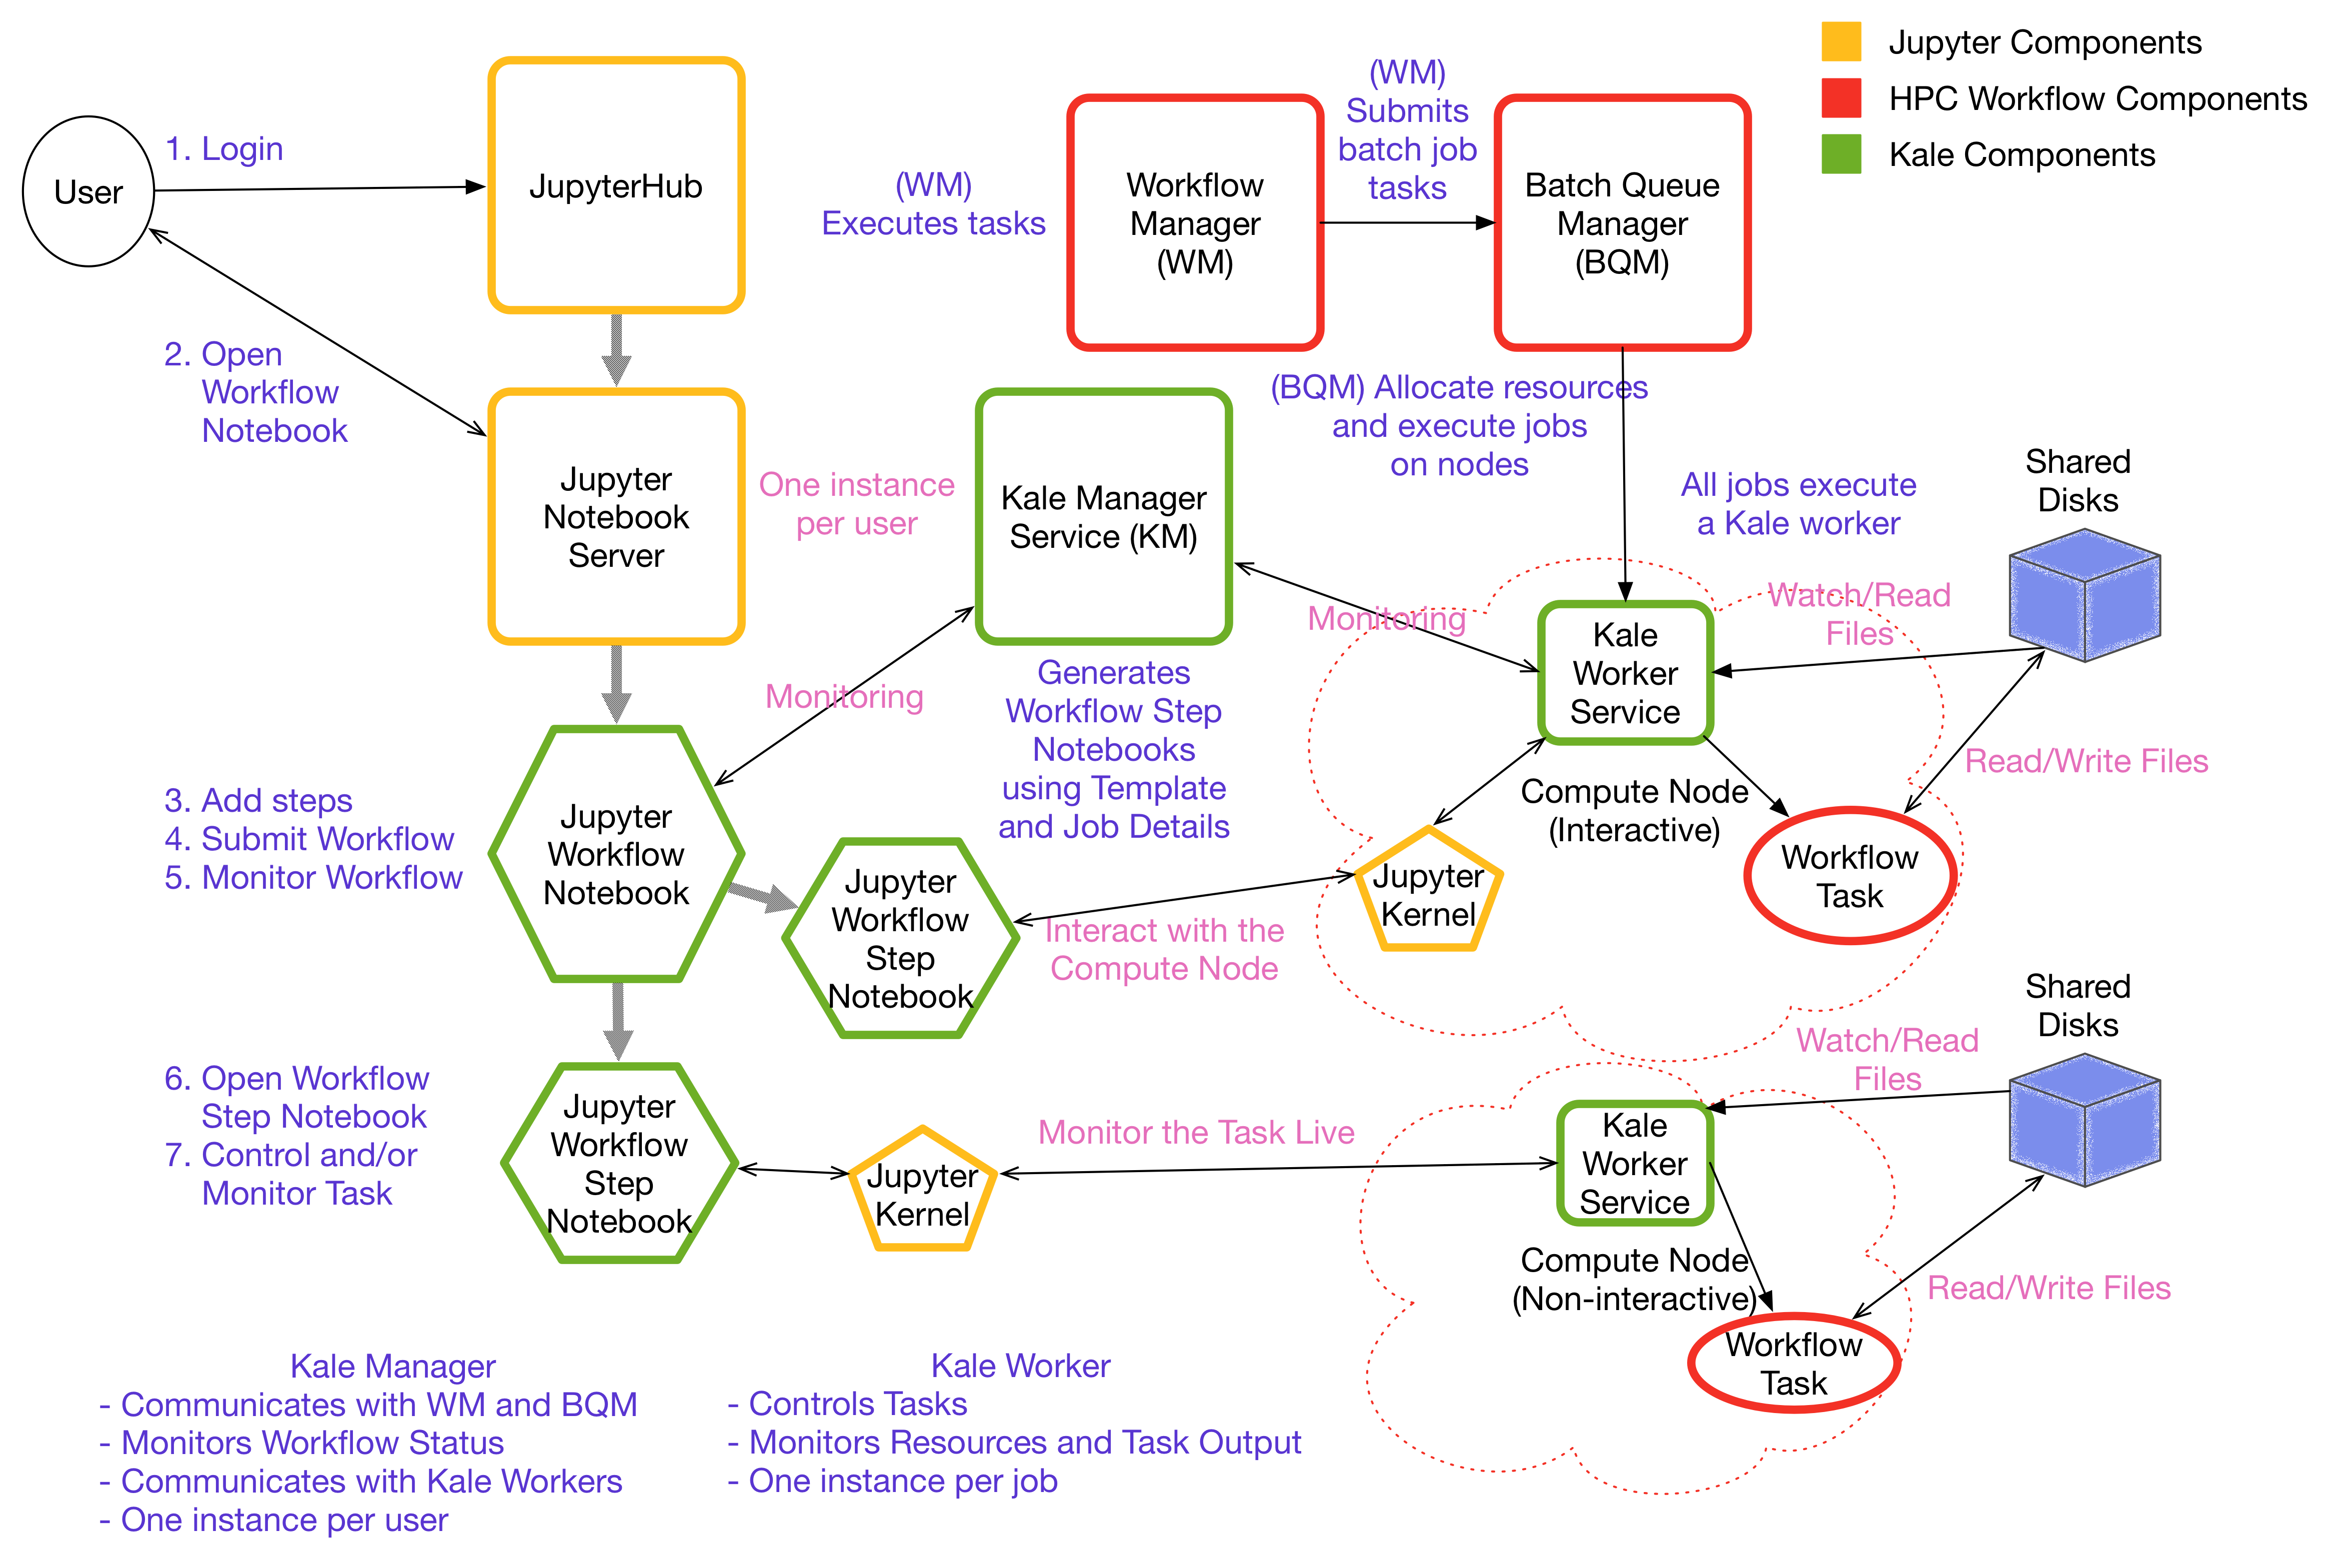
\includegraphics[width=\linewidth]{Kale_HPC}
 }
 
\column{0.3}

\block{Define Workflows} {
    \begin{minipage}{.6\linewidth}
        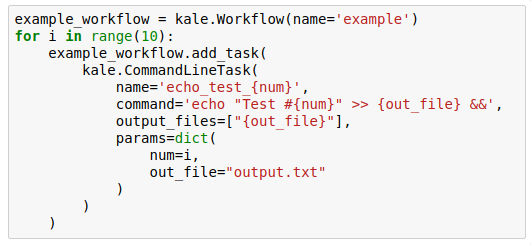
\includegraphics[width=\linewidth]{../img/screenshot/define} \\
    \end{minipage}
    \begin{minipage}{.39\linewidth}
        \begin{itemize}
            \item Define workflows via Python
            \item Simple API
            \item Refer to tasks by name
            \item Data provenance
            \item Easy parameter substitution
        \end{itemize}
    \end{minipage}

    \vspace{-1.5em}
}

\block{Visualize \& Run} {
    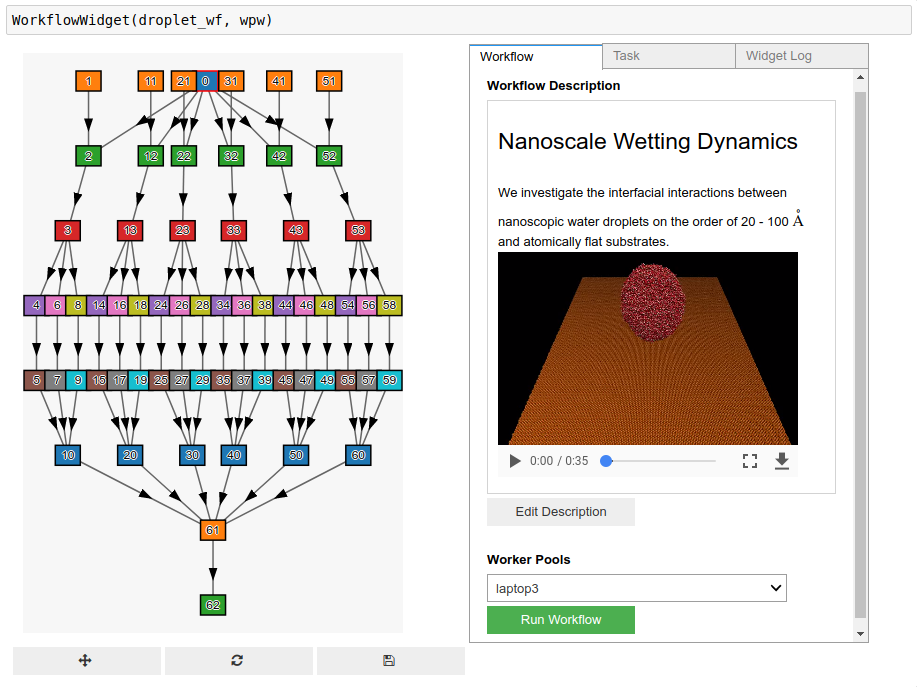
\includegraphics[width=\linewidth]{../img/screenshot/visualize_droplet}
}

\block{Observe Live Output} {
\begin{multicols}{2}
    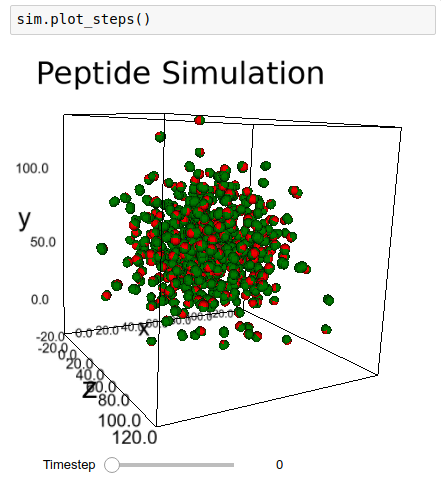
\includegraphics[width=\linewidth]{../img/screenshot/peptide} \\
    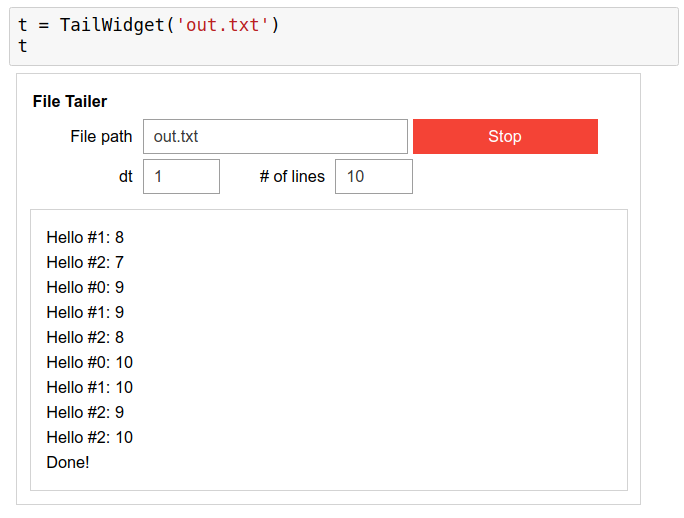
\includegraphics[width=.95\linewidth]{../img/screenshot/tail}
\end{multicols}
}


\column{0.25}

\block{Principles} {

Jupyter brings several key features to the world of computational
science: Exploration, Narrative, and Interactivity

While these are powerful qualities, Jupyter presently operates at the
level of an individual notebook in one language. We seek to harness the
power of Jupyter to bring these qualities to full scientific workflows,
which often involve many steps across a variety of languages.

\section*{Exploration}\label{exploration}

Scientists love to explore. But being constrained by computational
resources, scientific computing tends to focus on maximizing
computational efficiency, while sacrificing human involvement. By
combining the raw power of high performance computing resources with the
flexibility of Jupyter, we can go from idea to implementation in
minutes, even on the biggest problems.

\section*{Narrative}\label{narrative}

Having Markdown and LaTeX right next to your code allows you to tell the
full story of what's going on in a notebook in a clear and cohesive
manner. With formulas, images, tables, and even movies embedded right in
the document, communicating complex concepts is so much more feasible
than through code comments alone. While sharing code is essential for
open science and reproducibility, it usually doesn't go very far without
context.

By bringing the power of narrative from the individual notebook to full
workflows, we hope to make HPC workflows as easy to share effectively as
small individual notebooks.

\section*{Interactivity}\label{interactivity}

Being able to touch your data and models provides a deeper ability to
understand them. The Jupyter widget ecosystem provides a wide range of
interactive elements that allow for the visualization and exploration of
high dimensional spaces. In HPC systems, interactivity has generally
been at the bottom of the food chain. We hope to bridge that gap by
providing an easy means by which to examine simulations and analysis
codes as they run, and to be able to have interactive pieces of a
scientific workflow, where you know that you're going to need human
interaction in between computational tasks.

\block{Dashboard Widgets} {
\begin{itemize}
\tightlist
\item
  Workflow DAG visualizer/runner
\item
  Live updating plots/logs
  \item Local/remote worker creation
\item
  Batch queue status
\item
  Resource monitors
\item
  SSH/REST authenticators

\end{itemize}
}

\end{columns}


\end{document}
